\subsection{The TorPath Protocol}

\subsubsection{Overview}

We introduce the TorPath protocol for assigning Tor circuits to clients. It overrides Tor directory servers with \textit{assignment servers}, which form decentralized \textit{consensus groups}. The protocol guarantees that no participant on a circuit can identify all other participants, and that each circuit includes a publicly verifiable signature. We use TorPath to ``sign'' each TorCoin, so that anyone can verify its authenticity.

\subsubsection{Requirements}

The TorPath protocol adheres to the following constraints:

\begin{itemize}
  \item No client can generate its own circuit.
  \item Every circuit has a unique, publicly-verifiable signature.
  \item No client can know the circuit of another client.
\end{itemize}

\subsubsection{Protocol Description}
At a high level, the TorPath protocol follows a simple algorithm:

\begin{enumerate}
\item A TorPath client requests a new circuit from an assignment server.
\item Assignment Ssrvers form a \textit{consensus group} upon client quorum.
\item They divide into three \textit{shuffle sets}, each responsible for a different relay on the circuit.
\item Each shuffle set performs a Neff shuffle on its list of relays.
\item Assignment Servers notify clients of new circuits.
\end{enumerate}

Next we will descibe the consensus groups and Neff shuffle in more detail.

\begin{figure}[H]
  \centering
    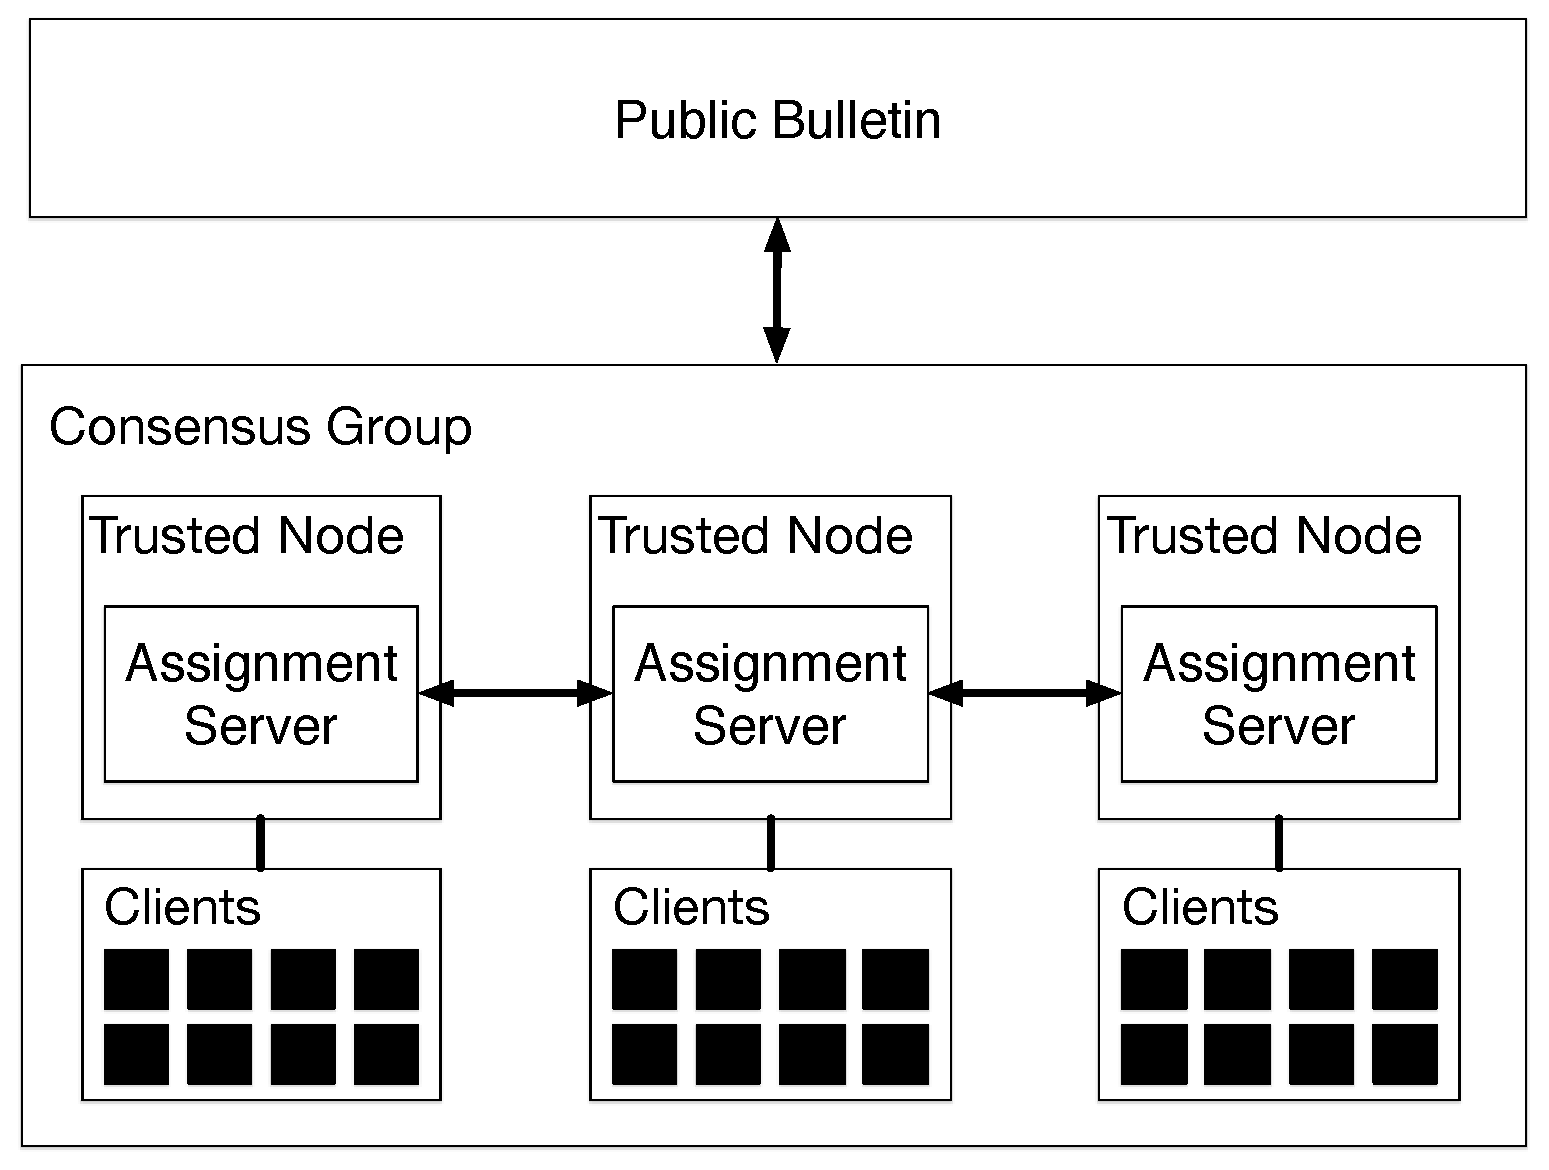
\includegraphics[scale=0.3]{torpath_grouping.pdf}
  \caption{TorPath Consensus Group Formation.}
\end{figure}

\subsubsection{Group Formation}
An assignment server joins a group when it reaches a sufficient number of clients. In practice, we expect the number to be modulated so that groups are being created every 10 seconds or so. To ensure diversity, groups must include a majority of the assignment servers on the network. For example, if there are ten of assignment servers on the entire network, a consensus group requires at least six.

Once a consensus group exists, it splits into three decentralized shuffle sets, each responsible for assigning a different relay to clients. An $n$-client shuffle set has $n$ rows, each pointing to a possible relay. For example, shuffle sets $s_0$, $s_1$, and $s_2$ could be responsible for assigning entry, middle, and exit relays to clients. 

\subsubsection{Neff Shuffles for Circuit Assignment}
Each shuffle set runs a Neff shuffle ~\cite{neff2001verifiable} to shuffle its list of $n$ relays, so that it can assign each relay $i$ to client $i$. Each client receives a tuple $(r_0, r_1, r_2, s)$ specifying the address of entry, middle, and exit relays, along with a circuit signature.

\begin{figure}
  \centering
    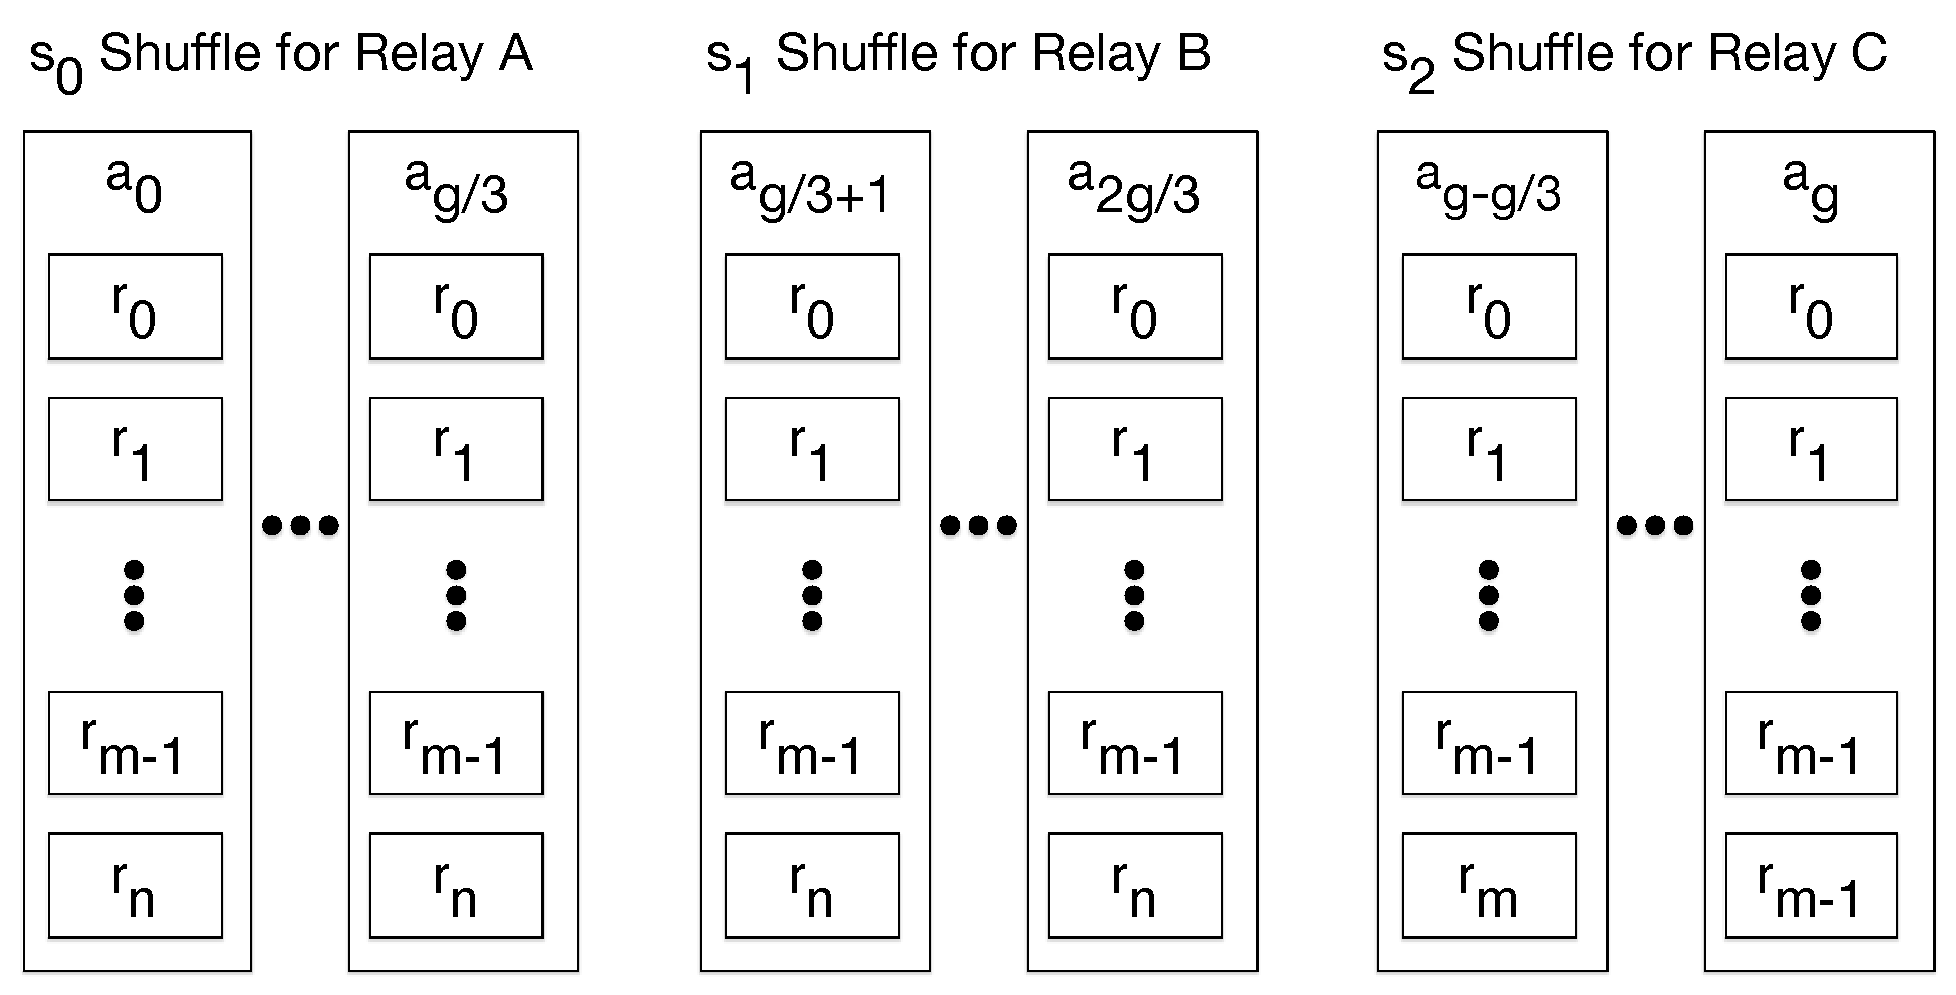
\includegraphics[scale=0.3]{torpath_shufflesets.pdf}
  \caption{Each Shuffle Set carries out its own Neff shuffle to determine one part of the path.}
\end{figure}

\subsubsection{TorCoin Verification}
Assignment servers input circuit signatures into a cryptographic accumulator, and publish that list of accumulators. Anyone can verify that a circuit existed at least once, simply by searching for a signature.

\subsubsection{Circuit Anonymity}
The TorPath protocol guarantees that no single server can be aware of the entire circuit of any client. Since each point in the circuit is confirmed by at least two assignment servers, it is also robust to rogue attacks.

\subsubsection{Decoupled Protocol}
The TorPath protocol only replaces directory servers. Therefore, implementing it does not require modifying any Tor code. So clients can use the TorPath protocol for circuit assignment then communicate using the existing Tor protocol.